\subsection{Overall accuracy of Simplified Ikeda method}
\label{se:overall_comparison}
An investigation of how well the implementation of the Simplified Ikeda method (see section \ref{se:semi-empirical methods}) agree with the corresponding result in the roll damping database has been carried out. 

To enable a comparison the equivalent linear damping coefficient is used \parencite{himeno_prediction_1981}:
\begin{equation}
B_{e} = B_{1} + \frac{8 B_{2} \omega_{0} \phi_{a}}{3 \pi}
\end{equation}


For the roll damping database $B_1$ and $B_2$ can be inserted directly into equation  \ref{eq:B_e_equation}. 
In order to obtain the same coefficients for the simplified Ikeda's method, roll damping is calculated for two or more roll amplitudes $\phi_a$ for the same motion frequency (for this study, it is referred to the natural frequency $\omega_0$ because free roll decay tests were used for the model tests.). $B_1$ and $B_2$ is obtained by fitting equation \ref{eq:B_e_equation} to this data.  

$\hat{B_e}$ is the non-dimensional equivalent linear damping coefficient \parencite{himeno_prediction_1981}.
Figure \ref{fig:B_e_hat_ikeda_zero} and \ref{fig:B_e_hat_ikeda} show a comparison of $\hat{B_e}$ from model tests and the simplified method where predicted damping with simplified Ikeda's method has been plotted against corresponding test in the roll damping database.  

\begin{figure}[H]
\centering
\begin{minipage}{.5\textwidth}
  \centering
  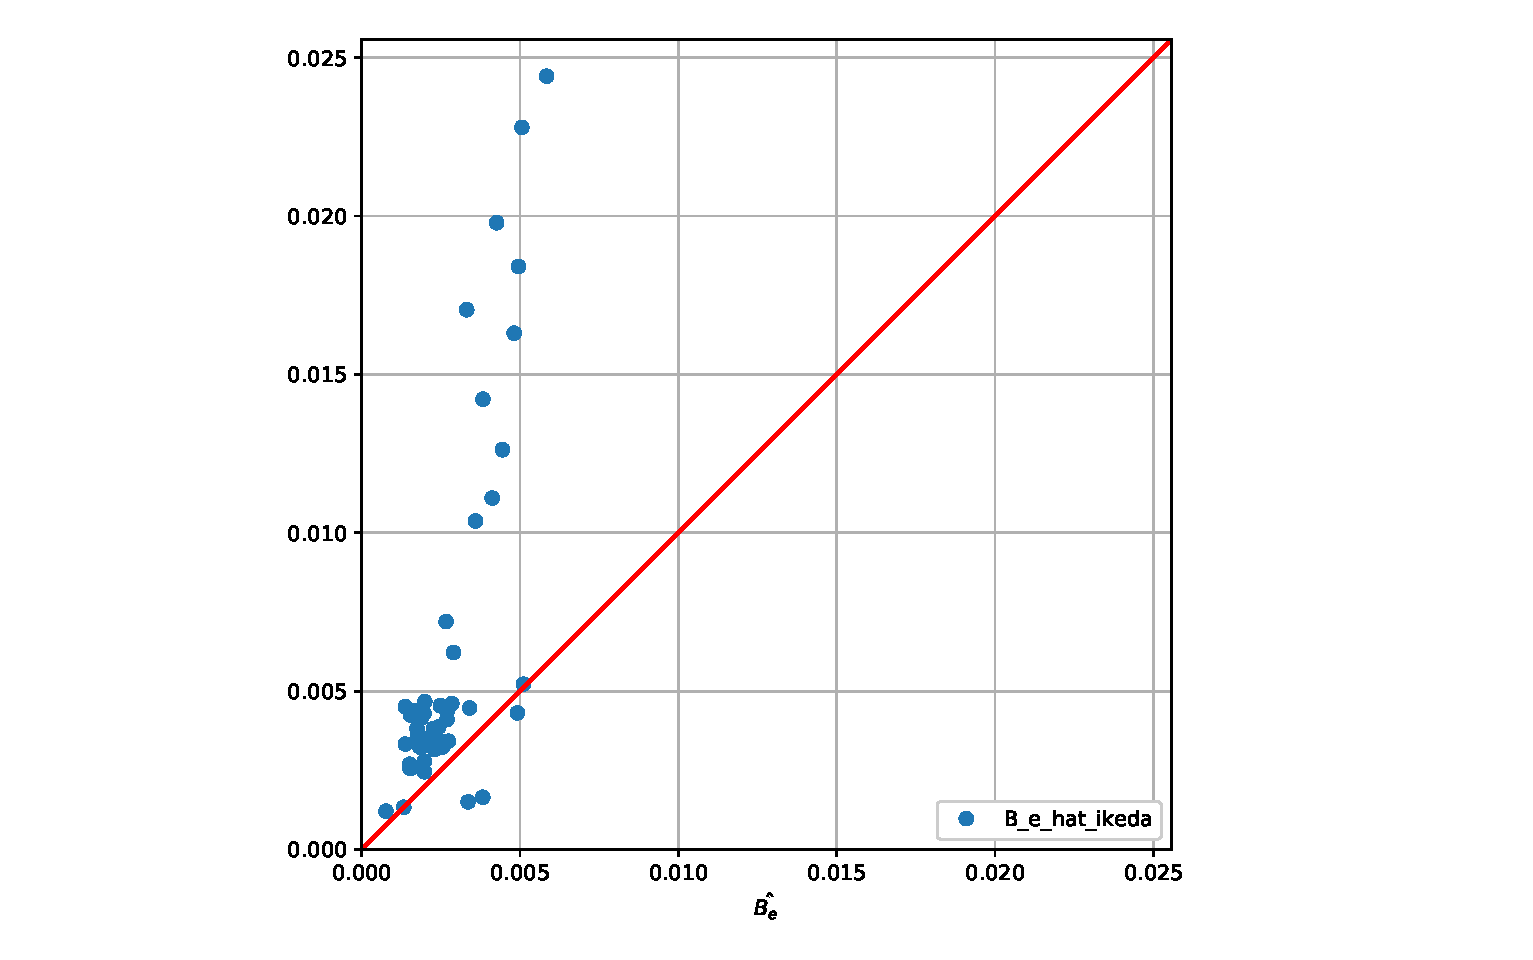
\includegraphics[width=1.0\columnwidth]{figures/B_e_hat_ikeda_zero.eps}
  \caption{$\hat{B_e}$ comparison at zero speed}
  \label{fig:B_e_hat_ikeda_zero}
\end{minipage}%
\begin{minipage}{.5\textwidth}
  \centering
  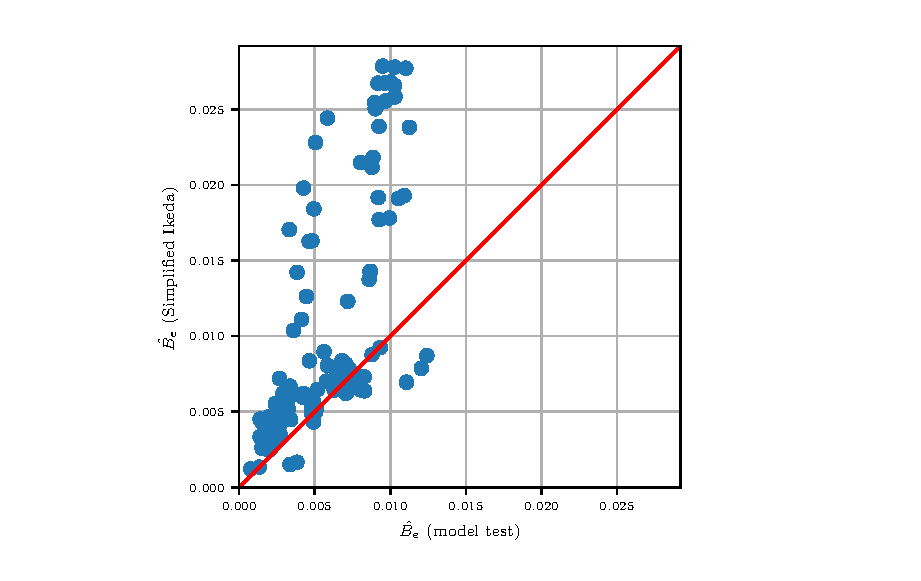
\includegraphics[width=1.0\columnwidth]{figures/B_e_hat_ikeda.eps}
  \caption{$\hat{B_e}$ comparison at all speeds}
  \label{fig:B_e_hat_ikeda}
\end{minipage}
\end{figure}


The comparison show poor agreement, both at speed and zero speed. The prediction error is highly dependent on the ship draught $T$, which is shown in figure  \ref{fig:B_e_hat_error}.
The figure shows that the error is much larger for $T/L_{pp}<0.034$. Also high frequencies ($\hat{\omega_0} > 0.6$) give larger errors.

\begin{figure}[H]
    \centering
    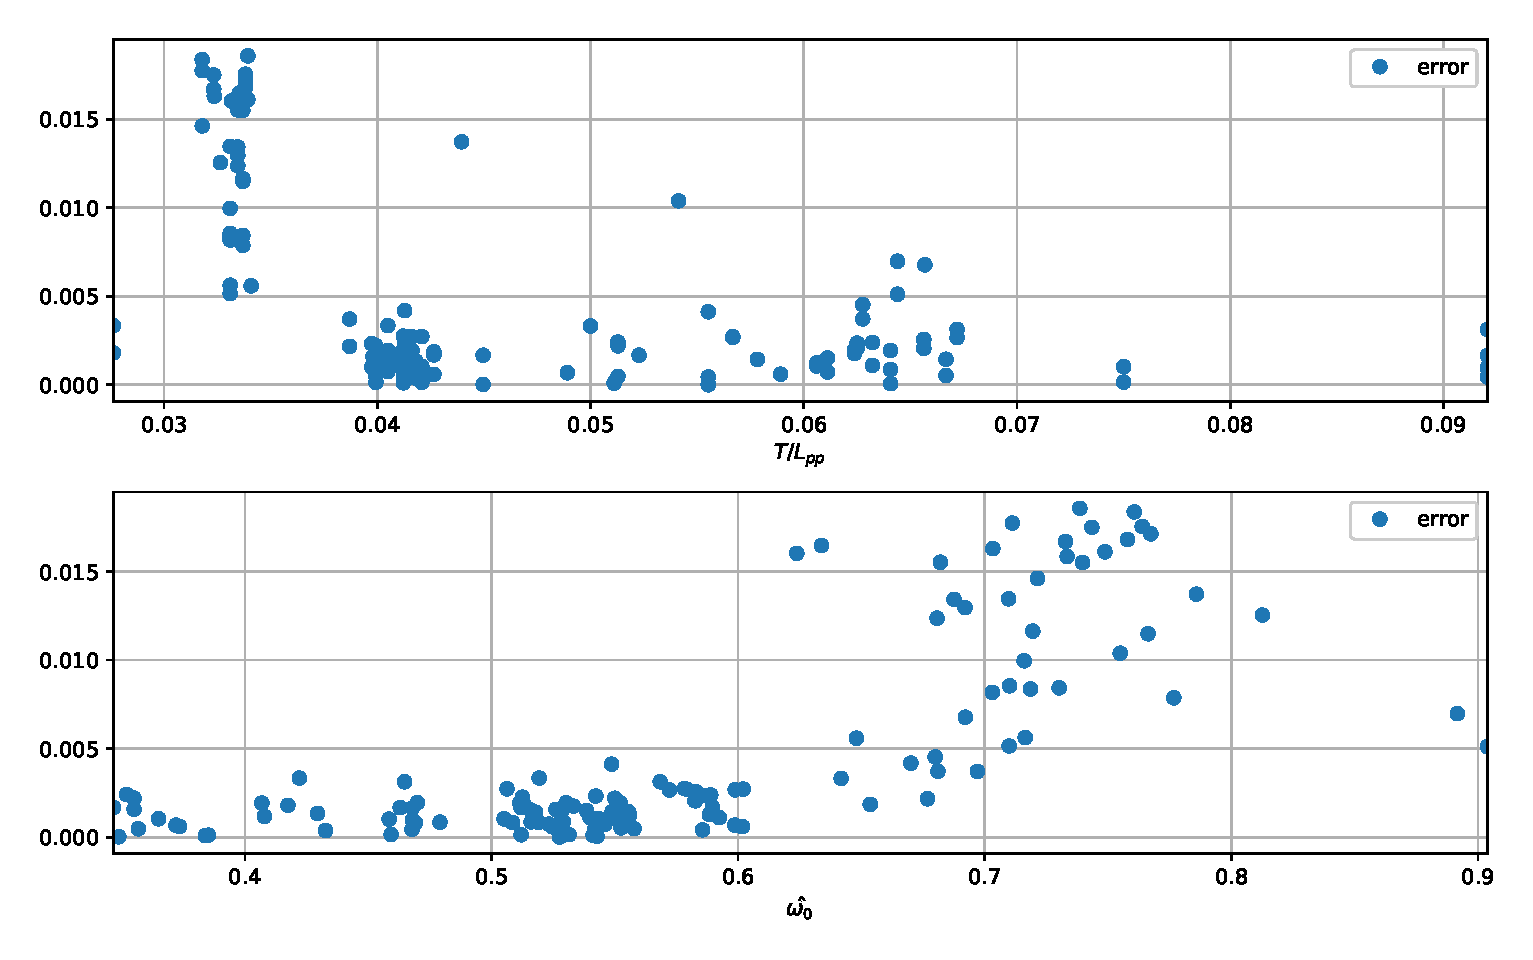
\includegraphics[width=0.9\columnwidth]{figures/B_e_hat_error.eps}
    \caption{Simplified Ikeda error versus draught}
    \label{fig:B_e_hat_error}
\end{figure}

\begin{figure}[H]
    \centering
    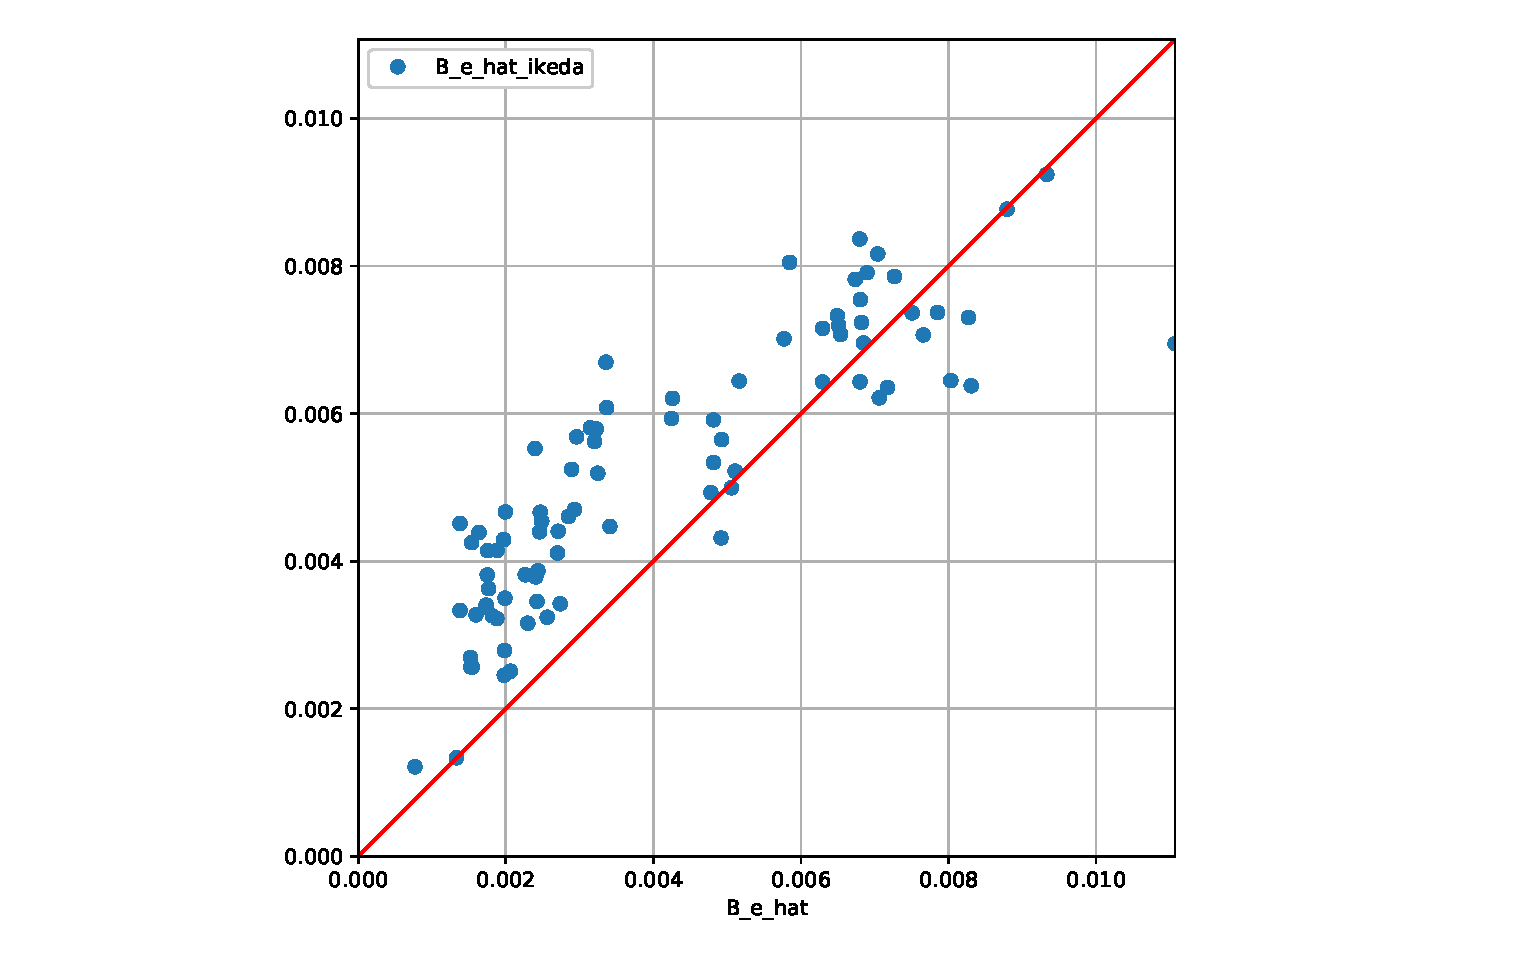
\includegraphics[width=0.9\columnwidth]{figures/B_e_hat_good.eps}
    \caption{$\hat{B_e}$ comparison with $T/L_{pp}>0.034$}
    \label{fig:B_e_hat_good}
\end{figure}

Figure \ref{fig:B_e_hat_good} shows the comparison for  model tests with $T/L_{pp}>0.034$ and $\hat{\omega_0} < 0.6$.
This confirms the small draft to beam ratio limit of this method as mentioned in \parencite{kawahara_simple_2011}. The corresponding $R^2$ score is 0.38.

\textcolor{red}{\subsection{Improved S1 in literature?}}

